\documentclass[11pt,a4paper]{amsart}
\usepackage[utf8]{inputenc}
\usepackage[T1]{fontenc}
\usepackage{lmodern}
\usepackage{amsmath,amssymb,amsthm}
\usepackage{graphicx}
\usepackage[margin=2.35cm]{geometry}
\usepackage{xcolor}
\usepackage[colorlinks=true,linkcolor=blue!50!black,citecolor=blue!50!black,urlcolor=blue!50!black]{hyperref}

\newtheorem{theorem}{Theorem}
\newtheorem{lemma}[theorem]{Lemma}
\newtheorem{proposition}[theorem]{Proposition}
\newtheorem{corollary}[theorem]{Corollary}
\theoremstyle{remark}
\newtheorem{remark}[theorem]{Remark}

\newcommand{\eg}{e^{-\gamma}}
\newcommand{\cA}{\mathcal{A}}
\newcommand{\PP}{\mathbb{P}}

\title[Limit points of normalized prime gaps]{A note on limit points of normalized prime gaps}
\author{Ruqing Chen}
\address{GUT Geoservice Inc., Montreal, Canada}
\email{ruqing@hotmail.com}
\date{April 2026}
\subjclass[2020]{11N05, 11N36}
\keywords{prime gaps, limit points, Maynard--Tao sieve, Erd\H{o}s--Rankin construction}

\begin{document}
\begin{abstract}
We revisit the paper of Banks, Freiberg and Maynard on limit points of normalized prime gaps
(Proc.\ London Math.\ Soc.\ 113 (2016)). We identify two gaps in the proofs and show how to close each of them;
the main theorems of that paper remain valid as stated.
(i) In Theorem~4.3(ii), which yields the result on chains of gaps, the main term with $8m^2+8m$ blocks and the
chosen parameters is exactly $0$ at its maximum, and the next term is smaller than the error terms. Moreover the
combinatorial step that follows needs pair weight $m+2$, not $m+1$. A different combinatorial conclusion, which is all the application
needs, works with weight $m$. Then $8m^2+1$ blocks suffice, so Theorem~1.3 holds as stated and in fact for any $8m^2+1$ numbers.
(ii) In the Erd\H{o}s--Rankin lemma (Lemma~5.2), with $z$ at the top of its range, the bracket claimed to be at least
$1-e^{-\gamma}$ tends to $1-4e^{-\gamma}<0$. The lemma is proved for $2z\le c\,y\log_2y/\log_3y$ with $c<e^\gamma/4$,
which suffices for the paper and for a later paper of Merikoski that quotes it.
\end{abstract}
\maketitle

\section{Introduction}

Let $d_n=p_{n+1}-p_n$ and let $\mathbb L$ be the set of limit points of $d_n/\log p_n$. Throughout, $\log_j$ denotes
the $j$-fold iterated logarithm and $\gamma$ is Euler's constant. Banks, Freiberg and Maynard
\cite{BFM} proved the following.
\begin{itemize}
\item Theorem~1.1: for any $\beta_1\le\dots\le\beta_9$ in $[0,\infty)$, some difference $\beta_j-\beta_i$ ($i<j$)
lies in $\mathbb L$. Hence (Corollary~1.2) $\lambda([0,T]\cap\mathbb L)\ge(1-o(1))T/8$, so at least $12.5\%$ of
nonnegative reals are limit points, and $\lambda([0,T]\cap\mathbb L)>T/22$ for all $T$ ($1/(8H_8)=0.04599\ldots$).
\item Theorem~1.3: for $m\ge2$ and any $\beta_1\le\dots\le\beta_k$ with $k=8m^2+8m$, some vector
$(\beta_{J(2)}-\beta_{J(1)},\dots,\beta_{J(m+1)}-\beta_{J(m)})$ with $J(1)<\dots<J(m+1)$ is a limit point of
$(d_n/\log p_n,\dots,d_{n+m-1}/\log p_{n+m-1})$.
\end{itemize}
Both rest on a Maynard--Tao sieve statement, Theorem~4.3, and on an Erd\H{o}s--Rankin construction, Lemma~5.2.
Theorem~4.3 is stated for $k$ a large multiple of $(8m+1)(8m^2+8m)$, a $k$-tuple $\cA$ and two partitions of
$\cA$ into $8m+1$ and $8m^2+8m$ equal blocks. Part~(i) gives $m+1$ blocks that contain primes; part~(ii) gives $m+1$
blocks with exactly one prime each and at most one prime in each block in between. Below, $\cA(n)\cap\PP$ is the set of primes
$n+h$, $h\in\cA$, $x=\rho\delta\log k$ with $0<\rho<1$ as in \cite[Lemma~4.6]{BFM}, and a block with $c$ primes
is called a singleton if $c=1$.

In brief, the two repairs are as follows. In Theorem~4.3(ii) we lower the weight attached to pairs of primes in a
common block from $w=m+1$ to $w=m$ and use $B=8m^2+1$ blocks instead of $8m^2+8m$; the main term is then strictly
positive, and a weaker combinatorial conclusion (Lemma~\ref{lem:comb}), which is all that the application requires,
replaces \cite[(4.21)]{BFM}. In Lemma~5.2 we restrict the upper end of the range of $z$ to
$2z\le c_0\,y\log_2y/\log_3y$ with a fixed constant $c_0<e^\gamma/4$, which keeps the Erd\H{o}s--Rankin bracket
positive and still covers every use of the lemma.

Section~\ref{sec:tie} treats Theorem~4.3(ii) and Section~\ref{sec:ER} treats Lemma~5.2.
Line numbers refer to the source of the arXiv version of \cite{BFM} (arXiv:1404.5094), and so does the numbering
of lemmas. All numbers are reproduced by a short program provided as supplementary material
(DOI~\href{https://doi.org/10.5281/zenodo.24315678}{10.5281/zenodo.24315678}).

\section{Theorem 4.3(ii) and the chains of gaps}\label{sec:tie}

\subsection{The main terms}
By \cite[Lemmas~4.5 and~4.6]{BFM}, a single prime contributes at least $x/k$ and a pair at most
$(4+O(\delta))(x/k)^2$, relative to $\frac NWB^{-k}I_k(F)$, with relative errors $O((\log k)^{-1/2})$.
In part~(i) (lines 1840--1899), with $x=2m$ and $8m+1$ blocks of size $k/(8m+1)$, the paper finds the main term
$\frac m{8m+1}+\frac{8m^2}k+O(\delta)$. This is correct when the inner sum runs over \emph{unordered} pairs
$h\ne h'$. Over ordered pairs it would be $\frac{m-8m^2}{8m+1}+\frac{16m^2}k<0$.

In part~(ii) (lines 1901--1947) the weight is $\sum_i\mathbf 1_\PP(n+h_i)-m-w\sum_j\sum_{\{h,h'\}\subset\cA_j}\mathbf
1_\PP(n+h)\mathbf 1_\PP(n+h')$ with $w=m+1$ and $B=8m^2+8m$ blocks. (From here on $B$ denotes the number of blocks,
except in the normalising factor $\frac NWB^{-k}I_k(F)$, where it is the quantity so named in \cite[\S4]{BFM}.)
The same computation gives
\begin{equation}\label{eq:f}
\frac{S'}{\frac NWB^{-k}I_k(F)}\ \ge\ f_{w,B}(x)+\frac{2wx^2}k+O\bigl(\delta+(\log k)^{-1/2}\bigr),\qquad
f_{w,B}(x)=x-m-\frac{2wx^2}{B}.
\end{equation}
The maximum of $f_{w,B}$ is $B/(8w)-m$, at $x=B/(4w)$. For $w=m+1$ and $B=8m(m+1)$ we get $f(x)=-(x-2m)^2/(4m)$, so
the maximum is exactly $0$, at the paper's choice $x=2m$. The remaining term $8m^2(m+1)/k$ is smaller than the error,
because $\delta=x/(\rho\log k)>2m/\log k$. Thus $S'>0$ is not established (Figure~\ref{fig:audit}(a)). With
$B=8m^2+8m+1$ blocks the maximum would be $1/(8(m+1))>0$, and $f(2m)=m/B$.

\subsection{The combinatorial step}
Increasing $B$ does not complete the proof. If $n$ contributes positively to $S'$, the paper
(lines 1931--1942) claims that at least $m+1+mr$ blocks are singletons, where $r$ is the number of blocks with two or
more primes, and deduces \cite[(4.21)]{BFM}. But with $w=m+1$ a block with two primes contributes $2-(m+1)=1-m$, so
one only gets $m+1+(m-1)r$. For example, the block pattern $(1,\dots,1,2,1,\dots,1)$ with $m$ singletons on each side
gives $2m+2-m-(m+1)=1>0$, yet no $m+1$ singletons are free of the block with two primes between them.
The count $m+1+mr$, and with it (4.21), holds for $w=m+2$. That requires
$B>8m(m+2)$, i.e.\ $8m^2+16m+1$ blocks. This is the case $r=2$ of the threshold of Lau \cite{Lau}, whose
weight $m(r-1)+r$ equals $m+2$ when $r=2$.

The deduction in \cite[\S6]{BFM} does not need (4.21), however. It needs only $m+1$ \emph{consecutive} primes of
$\cA(n)\cap\PP$ in $m+1$ distinct blocks. For this the weight $w=m$ is enough.

\begin{lemma}\label{lem:comb}
Let $m\ge2$, let $c_1,\dots,c_t\ge1$ be integers, and suppose $\sum_ic_i-m-m\sum_i\binom{c_i}2>0$. Then there is
$a$ with $0\le a\le t-m-1$ and $c_{a+2}=\dots=c_{a+m}=1$. The weight $m$ cannot be lowered: for $w<m$ the
sequence $(1^{m-1},2,1^{m-1})$ has positive weight $\sum_ic_i-m-w\sum_i\binom{c_i}2$ and no such $a$.
\end{lemma}

\begin{proof}
Call the $i$ with $c_i\ge2$ heavy, let $r$ be their number, and $s=t-r$. Each heavy $i$ contributes
$c_i-m\binom{c_i}2\le2-m$. If $r=0$ then $t=s>m$ and $a=0$ works. Let $r\ge1$ and suppose no $a$ exists. Then a run
of singletons between two heavy indices has length at most $m-2$. A run at either end has length at most $m-1$.
Hence $s\le2(m-1)+(r-1)(m-2)$, and the weight is at most $s+r(2-m)-m\le0$, a contradiction.

For the example, $t=2m-1$ and the only heavy index is $i=m$, with $c_m=2$. Its weight is
$\bigl(2(m-1)+2\bigr)-m-w\binom22=m-w$, which is positive for $w<m$. On the other hand $0\le a\le t-m-1=m-2$ gives
$a+2\le m\le a+m$, so every window $\{a+2,\dots,a+m\}$ contains the heavy index $m$, and no admissible $a$ exists.
\end{proof}

\begin{proposition}[corrected Theorem~4.3(ii)]\label{prop:43}
Let $m\ge2$, $B=8m^2+1$, and let $k$ be a sufficiently large multiple of $B$. Assume the hypotheses of
\cite[Theorem~4.3]{BFM}, the second partition being $\cA=\cA_1\cup\dots\cup\cA_B$ into equal blocks with
$\max\cA_j<\min\cA_{j+1}$. Then there are $n\in(N,2N]$, $n\equiv b\bmod W$, and $J(1)<\dots<J(m+1)$ such that
$\cA(n)\cap\PP$, listed in increasing order, has $m+1$ consecutive elements lying in
$\cA_{J(1)}(n),\dots,\cA_{J(m+1)}(n)$ respectively.
\end{proposition}

\begin{proof}
Take the weight of part~(ii) with $w=m$ and $x=2m$. By \eqref{eq:f} the main term is
$f_{m,B}(2m)=m/(8m^2+1)>0$ (the maximum, at $x=B/(4m)$, is $1/(8m)$). So $S'>0$ for $k$ large and $\delta$ small.
For a positive $n$, list the non-empty blocks in increasing order with their prime counts $c_1,\dots,c_t$. As the
blocks are ordered as integers, $\cA(n)\cap\PP$ lists them block by block. Lemma~\ref{lem:comb} gives $a$; the last prime of
block $a+1$, the singletons $a+2,\dots,a+m$ and the first prime of block $a+m+1$ are consecutive.
\end{proof}

In \cite[\S6]{BFM} the blocks are ordered as integers provided the $h_i$ in \cite[Lemma~5.2]{BFM} are chosen
increasing in $i$, which is possible (each interval $(u_i,u_i+\Delta]$ contains at least $k$ admissible primes, and
equal $\beta_i$ give equal $u_i$). The conclusion of Proposition~\ref{prop:43} is exactly what the deduction of
\eqref{eq:f21} needs:
\begin{equation}\label{eq:f21}
\frac{p_{r+i+1}-p_{r+i}}{\log p_{r+i}}=\beta_{J(i+1)}-\beta_{J(i)}+o(1)\qquad(1\le i\le m).
\end{equation}
Hence \emph{Theorem~1.3 holds for any $8m^2+1$ nonnegative reals}, a fortiori for $8m^2+8m$. Theorem~4.3 holds with
$k$ a multiple of $(8m+1)(8m^2+1)$, and \S6.1 needs $k$ a multiple of $8m^2+1$ only.
For $m=1$ the window is any two non-empty blocks, weight $1$ suffices, and $B=9$: this is Theorem~1.1. We have not
checked whether the bound $8m^2+1$ appears in the later literature.

\emph{Theorem~1.1.} Its deduction (line~2688) takes $k$ a multiple of $9\times17$, which is not a multiple of
$(8m+1)(8m^2+8m)=9\times16$ for $m=1$. This is harmless: only part~(i) is used, which needs $9\mid k$.
In part~(i), (4.20) should read $|\cA_i^{(1)}(n_1)\cap\PP|\ge1$; the proof gives only this, since for $m=1$ two blocks
with two primes each have weight $4-1-2>0$. The deduction at lines~2695--2698 uses $\ge1$.

\section{The Erd\H{o}s--Rankin bracket in Lemma 5.2}\label{sec:ER}

In the proof of \cite[Lemma~5.2]{BFM} the number of primes in $(y_2,y]$ exceeds the number of uncovered integers by
at least (5.16) (lines 2353--2365):
\begin{equation}\label{eq:bracket}
\frac y{\log y_2}\Bigl(1-2\eg\frac{z\log(z/y_2)}{y\log y_1}\Bigr)+O\Bigl(\frac{y_2}{\log y_2}+\frac z{\log y_1\log y_2}\Bigr).
\end{equation}
Then (lines 2367--2381) $y_1=(\log y)^{1/4}$, $y_2=y/\log_3y$ and $y<2z\le y\log_2y/\log_3y$, and the bracket is
asserted to be at least $1-\eg$.

\begin{proposition}\label{prop:ER}
Let $2z=c\,y\log_2y/\log_3y$ with $0<c\le1$ fixed. Then the bracket in \eqref{eq:bracket} equals
$1-4c\,\eg+o(1)$. Its limit is negative for $c>e^\gamma/4=0.44527\ldots$. At $c=1$, the choice made in
\cite[\S6]{BFM} (line~2552), it tends to $1-4\eg=-1.24584\ldots$. The printed value $1-\eg=0.43854\ldots$ is the
limit at $c=1/4$.
\end{proposition}

\begin{proof}
We have $\log y_1=\frac14\log_2y$, $z/y=c\log_2y/(2\log_3y)$ and $z/y_2=\frac c2\log_2y$, so
$\log(z/y_2)=\log_3y+O(1)$. The subtracted term is
$2\eg\cdot\frac{c\log_2y}{2\log_3y}\cdot\frac{\log_3y+O(1)}{\frac14\log_2y}=4c\,\eg+o(1)$.
\end{proof}

Since $y_1\le C\sqrt{\log y}$ is forced by the use of Page's theorem (line 2367), $\log y_1\le\frac12\log_2y+O(1)$,
and the bracket stays negative at $c=1$ for every admissible $y_1$. The proof of Lemma~5.2 is therefore incomplete
near the top of its $z$-range, and the application in \S6 uses that end.

\emph{Repair.} Fix $c_0<e^\gamma/4$ and replace the upper condition in (5.5) by $2z\le c_0\,y\log_2y/\log_3y$.
Since $z\log(z/y_2)$ increases with $z$, the bracket is at least $1-4c_0\,\eg+o(1)>0$ uniformly in $z$. Any fixed
constant $c_0$ strictly less than $e^\gamma/4=0.44527\ldots$ is admissible. For definiteness one may take $c_0=2/5$,
for which the bracket is at least $1-\frac85\eg+o(1)$ with $1-\frac85\eg=0.10166\ldots$; alternatively $c_0=1/4$
gives exactly the constant $1-\eg$ printed in \cite{BFM}. The
conditions $z<y_1y_2$, $2\log y_1\le\log z/\log_2z$ and $\log(z/y_2)<\log y_1$ still hold, so the rest of the proof is
unchanged; $y(\boldsymbol\beta,k)$ now also depends on $c_0$. In \S6, $x=\epsilon^{-1}$ is fixed and the only lower
requirement is $z\ge y(1+(1+\beta_k)x)$. So one may take $z=y(1+(1+\beta_k)x)$, a fixed multiple of $y$ (then
the bracket tends to $1$), or $z=c_0y\log_2y/(2\log_3y)$.

\emph{The remark at line 2744.} There $\log N$ in \eqref{eq:f21} is replaced by $f(N)$ with $f(N)/\log N$ growing
as fast as $\log_3N/\log_4N$. This means $h_i\approx\beta_ixy$ with $xy=f(N)$ and $y=\epsilon\log N$. The lower
condition in (5.5) then forces $z/y\ge(1+\beta_k)f(N)/(\epsilon\log N)$, while $z/y\le\frac{c_0}2\log_2y/\log_3y$ and
$\log_2y\sim\log_3N$, $\log_3y\sim\log_4N$. So the remark needs $z$ of the order of the top of the range, which the
repaired lemma still allows. The growth rate $\log_3N/\log_4N$ therefore survives up to a constant factor. We
checked only this constraint, not the rest of the remark.

\emph{Merikoski.} Merikoski \cite{Mer} quotes \cite[Lemma~5.2]{BFM} verbatim with the same $z$-range and takes
$z=y(\log_2y)(2\log_3y)^{-1}$, again $c=1$ (lines~845--868 of arXiv:1811.03008), with $x=1/\epsilon$ fixed. The same
remark and the same repair apply. We have not examined the rest of \cite{Mer}. The lemma is also adapted in \cite{Lau}.

\begin{figure}[t]
\centering
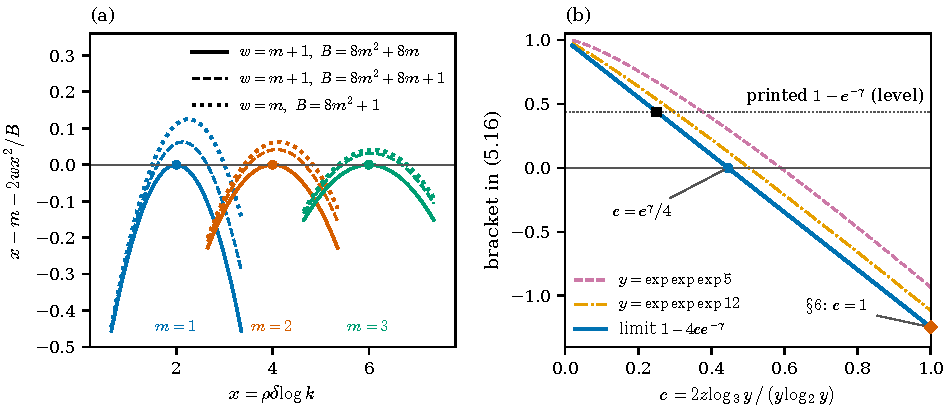
\includegraphics[width=0.86\textwidth]{figures/fig_bfm_2016_audit.pdf}
\caption{(a) The leading part $f_{w,B}(x)=x-m-2wx^2/B$ of the normalised main term of $S'$ in Theorem~4.3(ii),
for $m=1,2,3$. Solid: the paper's $w=m+1$, $B=8m^2+8m$; the curve touches $0$ at $x=2m$ (dots) from below. Dashed:
$w=m+1$, $B=8m^2+8m+1$. Dotted: the repair $w=m$, $B=8m^2+1$ of Proposition~\ref{prop:43}. The terms
$O(\delta)$ and $O((\log k)^{-1/2})$ in \eqref{eq:f} have no explicit constants in \cite{BFM} and are not plotted;
neither is $S'$ as a function of $k$.
(b) The bracket of \eqref{eq:bracket} for $2z=c\,y\log_2y/\log_3y$: the limit $1-4c\,\eg$ (solid), with its zero at
$c=e^\gamma/4$, and the exact bracket at $y=\exp\exp\exp t$, $t=5,12$. Dotted: the printed level $1-\eg$, which the
limit attains at $c=1/4$ (square). The paper uses $c=1$ (diamond).}
\label{fig:audit}
\end{figure}

\section{Numerical verification and scope}

The supplementary program (Python with \texttt{mpmath}) checks the following.
\begin{itemize}
\item Part~(i): exact rational main terms for $m\le5$; unordered pairs reproduce $\frac m{8m+1}+\frac{8m^2}k$, ordered
pairs give $\frac{m-8m^2}{8m+1}+\frac{16m^2}k$.
\item Part~(ii): for $m\le6$, $\max f=0$ for $(w,B)=(m+1,8m^2+8m)$; $\max f=\frac1{8(m+1)}$ and $f(2m)=\frac m{8m^2+8m+1}$
for $B=8m^2+8m+1$; $\max f=\frac1{8m}$ for $(m,8m^2+1)$.
\item Lemma~\ref{lem:comb}: all $3^t$ sequences $c_i\in\{1,2,3\}$, $t\le13$, for $m=2,3,4$. With $w=m$ and $w=m+1$
the window always exists; (4.21) fails for $w=m+1$ (first case $(1,1,2,1,1)$ at $m=2$) and holds for $w=m+2$.
For $w=m-\frac12$ the window fails, first at $(1,2,1)$ for $m=2$.
\item The bracket along $y=\exp\exp\exp t$: at $c=1$ it equals $-0.857$, $-1.168$, $-1.242$ for $t=4,20,400$; at
$c=1/4$ it decreases to $0.4385\ldots$; at $c=e^\gamma/4$ it is positive and tends to $0$
(Figure~\ref{fig:audit}(b)).
\end{itemize}

\enlargethispage{2\baselineskip}%
\subsection*{Scope} The analytic inputs (Lemmas~4.1, 4.4--4.6 and the modified Bombieri--Vinogradov theorem) were
not re-examined, and nothing beyond its use of Lemma~5.2 was checked in \cite{Mer}. Minor misprints in \cite{BFM}:
line~1813, $F_k(\rho\delta t_1,\dots)$ should be $F_k(t_1/(\rho\delta),\dots)$, as the scaling factors $(\delta\rho)^k$
show; line~2389, ``Lemma~5.2'' should be Lemma~5.1; line~2645, $p\in\mathcal Z$ should be $p\notin\mathcal Z$;
line~2697, the second $\cA_i$ should be $\cA_j$. At line~287 the range $j\le\kappa$ is correct ($\kappa$ numbers have
differences $\alpha,\dots,(\kappa-1)\alpha$), but the hats clash with the $(\kappa-1)$-term sequence defined above.

\begin{thebibliography}{9}
\bibitem{BFM} W.~D.~Banks, T.~Freiberg and J.~Maynard, \emph{On limit points of the sequence of normalized prime gaps},
Proc.\ London Math.\ Soc.\ (3) \textbf{113} (2016), no.~4, 515--539, DOI~10.1112/plms/pdw036; arXiv:1404.5094.
\bibitem{Lau} C.~F.~Lau, \emph{Residue class patterns of consecutive primes}, Acta Arith., online first (2026),
DOI~10.4064/\allowbreak aa240925-22-9; arXiv:2409.12819.
\bibitem{Mer} J.~Merikoski, \emph{Limit points of normalized prime gaps}, J.\ London Math.\ Soc.\ (2) \textbf{102}
(2020), no.~1, 99--124, DOI~10.1112/jlms.12314; arXiv:1811.03008.
\end{thebibliography}
\end{document}
